Esta sección corresponde a los resultados obtenidos con el problema descrito como ejemplo en la página web tutorial de Qiskit\cite{qiskit_tutorial_antiguo}, replicado en la \textit{sección~\ref{sec:4-tutorial_de_qiskit}}.

Dada la naturaleza del problema Max-Cut existen siempre al menos dos resultados (en este caso ``1010'' y ``0101'') que devuelven el máximo de la función de coste ($f(x) = 4$).
Un resultado ``1010'' sería equivalente a dar un valor ``1'' al nodo 3, ``0'' al nodo 2 y así sucesivamente.

\subsection{Resultados con QAOA}

Las estadísticas obtenidas son las siguientes:

\begin{table}[Resultados QAOA {--} max-cut en grafo de 4 aristas]{tab:5-tutorial-qaoa-estadisticas}{Resultados de la ejecución del problema~\cite{qiskit_tutorial_antiguo}}
  \begin{tabular}{|c|r|r|}
    \hline
    \textbf{nº Capas} & \textbf{NA/TE} & \textbf{MM/TE} \\ \hline
    p = 1 & 100\% & 52.14\% \\ \hline
    p = 2 & 100\% & 98.17\% \\ \hline
    p = 3 & 100\% & 96.10\% \\ \hline
    p = 4 & 100\% & 98.70\% \\ \hline
    p = 5 & 100\% & 98.90\% \\ \hline
  \end{tabular}
\end{table}

Según esta tabla, se encuentra el camino óptimo con cualquier número de capas el 100\% de las ejecuciones.
\\
Analizando los resultados, se concluye que son inmejorables, ya que siempre se encuentra el resultado óptimo y aumentar el número de capas disminuye la aparición de otros valores en la ejecución del algoritmo.

Se ha representado la función gamma, que muestra el comportamiento de la energía en función del parámetro $\gamma$, para poder visualizar posibles mínimos locales que se pudieran encontrar al ejecutar el optimizador clásico:

\begin{figure}[Función gamma {--} max-cut en grafo de 4 aristas]{fig:5-tutorial-gamma_fun}{Función gamma de \textit{execute\_circuit()} (con $\beta = 1.0$ y variando $\gamma$)}
  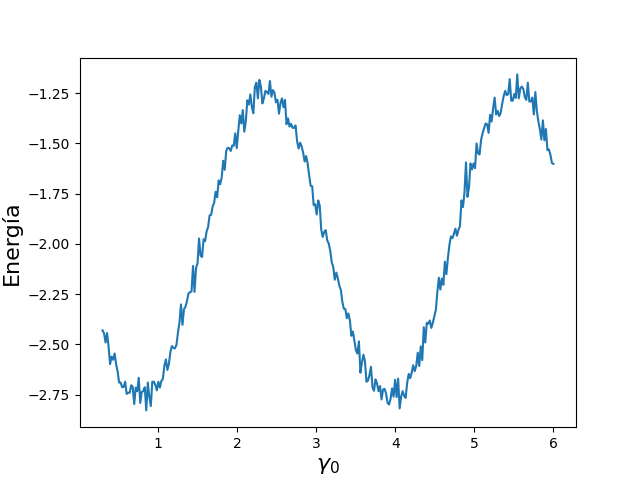
\includegraphics[scale=0.5]{qiskit-grafo/gamma-fun-2d.png}
\end{figure}

Como se puede ver, la función toma una forma sinusoidal y, como se verá posteriormente, tiene mucho menos ruido que otras ejecuciones.
Esto hace ver que el resultado óptimo es fácil de encontrar, lo que se ve reafirmado comprobando los resultados de la \textit{tabla~\ref{tab:5-tutorial-qaoa-estadisticas}}.

\subsection{Resultados de D-Wave}

El resultado de ejecutar el algoritmo de Quantum Annealing utilizando los sistemas de D-Wave es mostrado en la \textit{tabla~\ref{tab:5-tutorial-dwave_estadisticas}}.

\begin{table}[Resultados D-Wave {--} max-cut en grafo de 4 aristas]{tab:5-tutorial-dwave_estadisticas}{Resultados de la ejecución de max-cut en D-Wave}
  \begin{tabular}{|c|r|r|}
    \hline
    \textbf{Camino}        & \textbf{Energía} & \textbf{Muestras} \\ \hline
    0101 (\textbf{Óptimo}) & -4.0             & 618               \\ \hline
    1010 (\textbf{Óptimo}) & -4.0             & 406               \\ \hline
  \end{tabular}
\end{table}

Al igual que en la implementación de QAOA, que corresponde a los resultados de la \textit{tabla~\ref{tab:5-tutorial-qaoa-estadisticas}}, se obtienen unos resultados perfectos, ya que para el problema mencionado tanto \textit{0101} como \textit{1010} son los resultados óptimos.

\subsection{Resultados con librería de QAOA}

La \textit{tabla~\ref{tab:5-tutorial_qaoaansatz}} son estadísticas calculadas utilizando la función de Qiskit \textit{QAOAAnsatz}.

\begin{table}[Resultados QAOAAnsatz {--} max-cut en grafo de 4 aristas]{tab:5-tutorial_qaoaansatz}{Resultados utilizando \textit{QAOAAnsatz} con el problema de la \textit{fig.~\ref{fig:4-qiskit grafo}}}
  \begin{tabular}{|c|r|r|}
    \hline
    \textbf{nº Capas} & \textbf{NA/TE} & \textbf{MM/TE} \\ \hline
    p = 1 & 100\% & 51.30\% \\ \hline
    p = 2 & 100\% & 98.13\% \\ \hline
    p = 3 & 100\% & 95.83\% \\ \hline
    p = 4 & 100\% & 97.71\% \\ \hline
    p = 5 & 100\% & 99.50\% \\ \hline
  \end{tabular}
\end{table}

Esto ha sido realizado para comparar con la implementación de QAOA, cuyos resultados se muestran en la \textit{tabla~\ref{tab:5-tutorial-qaoa-estadisticas}}.
En ambas tablas se puede ver que siempre se ha encontrado el resultado óptimo y con el aumento de capas disminuye la aparición de otros resultados en el algoritmo en general.
\\
Con esta comparación se concluye que la implementación de QAOA de la \textit{sección~\ref{sec:4-tutorial_de_qiskit}} es correcta.


%%% Local Variables:
%%% mode: latex
%%% TeX-master: "../tfgtfmthesisuam"
%%% End:
